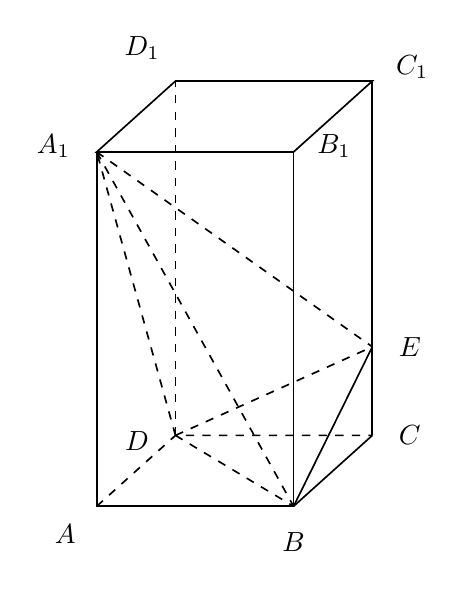
\begin{tikzpicture}[x=1cm,y=1cm,line width=.6pt,font=\normalsize]
% Schematic cuboid; tall prism, not metric
\coordinate (A) at (0,0);
\coordinate (B) at (2.5,0);
\coordinate (C) at (3.5,0.9);
\coordinate (D) at (1,0.9);
\coordinate (A1) at (0,4.5);
\coordinate (B1) at (2.5,4.5);
\coordinate (C1) at (3.5,5.4);
\coordinate (D1) at (1,5.4);
\coordinate (E) at (3.5,2.025);
% front face solid
\draw (A)--(B)--(B1)--(A1)--cycle;
% top face solid
\draw (A1)--(B1)--(C1)--(D1)--cycle;
% right face

\draw (C1)--(E)--(C);
\draw (B)--(C);

% hidden base/vertical edges
\draw[dashed] (A)--(D)--(C);
\draw[dashed] (D)--(D1);
\draw[dashed] (D)--(A1);
% hidden diagonals from A1

\draw[dashed] (A1)--(B);
\draw[dashed] (A1)--(E);
\draw[dashed] (D)--(B);
\draw[dashed] (D)--(E);
% solid edge B-E
\draw (B)--(E);
% labels with clearance
\node[anchor=north east,xshift=-4pt,yshift=-3pt] at (A) {$A$};
\node[anchor=north,yshift=-6pt] at (B) {$B$};
\node[anchor=west,xshift=6pt] at (C) {$C$};
\node[anchor=east,xshift=-6pt,yshift=-2pt] at (D) {$D$};
\node[anchor=east,xshift=-6pt,yshift=2pt] at (A1) {$A_{1}$};
\node[anchor=west,xshift=5pt,yshift=2pt] at (B1) {$B_{1}$};
\node[anchor=west,xshift=5pt,yshift=5pt] at (C1) {$C_{1}$};
\node[anchor=south east,xshift=-2pt,yshift=4pt] at (D1) {$D_{1}$};
\node[anchor=west,xshift=6pt] at (E) {$E$};
\end{tikzpicture}
